\documentclass{article}
\usepackage[utf8]{inputenc}
\usepackage{minted}
\usepackage{CJKutf8}
 

\begin{CJK}{UTF8}{}
 \CJKfamily{mj}

\title{Research Report}
\author{Image Lab, Min-Gi Yeom, Ha-Noung, Kwak }
\date{-Lab Date: 04/09/17      -Due Date: 07/12/17}
\end{CJK}

\usepackage{natbib}
\usepackage{graphicx}
\usepackage{indentfirst}\setlength\parindent{2em}

\begin{document}

\begin{CJK}{UTF8}{}
 \CJKfamily{mj}
\maketitle

\section{Research Plan}
      -Python study \newline
04/09/17 Planning, Role allocation\newline
05/09/17 Planning- Python study(www.codeacademy.com)\newline
06/09/17 Python study- chap 1, 2\newline
07/09/17 Python study- chap 3, 4\newline
11/09/17 Python study- chap 5, 6\newline
12/09/17 Python study- chap 7, 8\newline
13/09/17 Python study- chap 9, 10\newline
14/09/17 Python study- chap 11, 12\newline
15/09/17 Python study- chap 13\newline\newline

-Inflearn(https://www.inflearn.com) Machine Learning Lecture\newline
18/09/17 Inflearn -Machine Learning & TensorFlow\newline
19/09/17 1-1 Basic Machin Learning concept\newline
20/09/17 2-1 Linear Regression, Hypothesis and cost\newline
21/09/17 2-2 Implementation Linear Regression, Tensorflow\newline
22/09/17 3-1 cost Minimize algorithm of Linear Regression\newline
25/09/17 3-2 Implementation cost Minimize, Tensorflow\newline
26/09/17 4-1 Multi-variable Linear Regression\newline
27/09/17 4-2 Implementation Multi-varible Linear Regression, Tensorflow\newline
28/09/17 5-1 Logistic Classification, Hypothesis\newline
29/09/17 5-2 Logistic Regression, Cost function\newline
02/10/17 6-1 Multinomial(Softmax)\newline
03/10/17 6-2 Implementation Softmax classification, Tensorflow\newline
04/10/17 7-1 Learning rate, overfitting\newline
05/10/17 8-1 Basic concept of Deep Learning, XOR problem\newline
06/10/17 8-2 Backpropagation\newline
09/10/17 9-1 Initial weight\newline
10/10/17 9-2 Dropout\newline

-Break\newline
12/10/17 - 20/10/17 Midterm Exam)\newline

-PyTorchZeroToAll\newline
23/10/17 Basic concept of Machine Learning & Deep Learning\newline
24/10/17 PyTorch Overview\newline
25/10/17 Design model\newline
26/10/17 Finding weight that minimize error\newline
27/10/17 Finding weight that minimize error\newline
30/10/17 Updating weight in model which has 1 or more hidden layers\newline
31/10/17 PyTorch's gradient function\newline
01/11/17 Type of Activation Functions\newline
02/11/17 Type of Optimizers(1): step direction\newline
03/11/17 Type of Optimizers(2): step size\newline
06/11/17 Make Binary prediction model (Pass or Fail)\newline
07/11/17 Reading data size at once\newline
08/11/17 Classify data to 3 or more\newline
09/11/17 CNN(1)\newline
10/11/17 CNN(2)\newline

-Application\newline
13/11/17 - 01/12/17 Deep Learning Application(1)\newline
04/12/17 - 27/12/17 Deep Learning Application(2)\newline


\section{Daily Report: Python study}
\subsection{06/09/17}
Python study\newline
-1. Python Syntax\newline
-2. String and Console Output\newline

\subsection{07/09/17}
Python study\newline
-3. Condtionals and Control Flow\newline
-4. Functions, Taking a Vacation\newline

\subsection{11/09/17}
Python study\newline
-5. Lists & Dictionaries, A Day at the Supermarket\newline
-6. Student Becomes the Teacher\newline

\subsection{12/09/17}
Python study\newline
-7. Lists & Functions, Battleship!\newline
-8. Loops, Practice Makes Perfect\newline

\subsection{13/09/17}
Python study\newline
-9. Exam Statistics\newline
-10. Advanced Topics in Python, Indtroduction to Bitwise Operators\newline

\subsection{14/09/17}
Python study\newline
-11. Introduction to Classes, Classes\newline
-12. File Input/Output\newline

\subsection{15/09/17}
Python study\newline
-13. Python Final Project\newline

\section{Daily Report: Inflearn, Machine Learning Lecture}
\subsection{18/09/17}
Inflearn -Machine Learning & TensorFlow\newline

\subsection{19/09/17}
1-1 Basic Machin Learning concept\newline
Supervised learning -learning with labeled examples(training sets)\newline
Unsupervised learning -unlabeled data(word clustering)\newline

@Common problem of Supervised Learning: \newline
Image labeling, Email spam filter, predicting exam score\newline
*	Predicting final exam score based on time spent(Regression)\newline
*	Pass/fail based on time spent (binary classification)\newline
*	Letter grade based on time spent (multi-label classification)\newline

\subsection{20/09/17}
2-1 Linear Regression, Hypothesis and cost\newline
Linear Regression, set the one Linear Hypothesis:  H(x)=Wx+b\newline
How fit the line to our (training) data : Cost(Loss) Function\newline

\begin{figure}[h!]
\centering
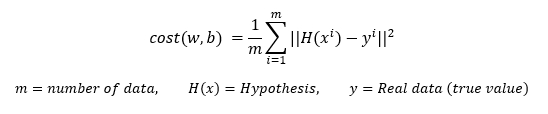
\includegraphics[scale=0.6]{1.jpg}
\end{figure}


Goal of the Linear Regression is Minimize the cost.\newline

\subsection{21/09/17}
2-2 Implementation Linear Regression, Tensorflow\newline
1.	build graph using TensorFlow operations\newline
2.	feed data and run graph(operation) > sess.run(op, feed_dict={x: x_data})\newline
3.	update variables in the graph(and return values)\newline

\subsection{22/09/17}
3-1 cost Minimize algorithm of Linear Regression\newline
Gradient descent algorithm : \newline
*	Minimize cost function\newline
*	Gradient descent is used many minimization problems\newline
*	For a given cost function, cost (W,b), it will find W,b to minimize cost\newline
*	It can be applied to more general function: cost(w1, w2, …)\newline

How it works?\newline
1.	Start with initial guesses, (0,0), Keeping changing W and b a little bit to try and reduce cost(W,b)\newline
2.	Each time you change the parameters, you select the gradient which redueces cost(W,b) the most possible\newline
3.	Repeat\newline
4.	Do so until you converge to a local minimum\newline
5.	Has an interesting property: Where you start can determine which minimum you end up\newline

\subsection{25/09/17}
3-2 Implementation cost Minimize, Tensorflow\newline
*	Gradient descent algorithm\newline
\begin{figure}[h!]
\centering
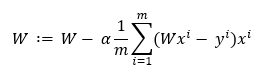
\includegraphics[scale=0.6]{2.jpg}
\end{figure}
\begin{minted}[mathescape,
               linenos,
               numbersep=5pt,
               gobble=2,
               frame=lines,
               framesep=2mm]{python}
#Minimize: Gradient Descent using derivative: W -= learning_rate * derivative
	Learning_rate = 0.1
	Gradient = tf.reduce_mean((W * X - Y) * X)
	Descent = W - learning_rate * gradient
	Update = W.assign(descent)
\end{minted}\newline

\subsection{26/09/17}
4-1 Multi-variable Linear Regression\newline
Set the hypothesis as\newline
\begin{figure}[h!]
\centering
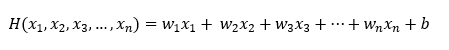
\includegraphics[scale=0.6]{3.jpg}
\end{figure}

Hypothesis using matrix\newline
H(X)=XW

\subsection{27/09/17}
4-2 Implementation Multi-varible Linear Regression, Tensorflow\newline
\begin{minted}[mathescape,
               linenos,
               numbersep=5pt,
               gobble=2,
               frame=lines,
               framesep=2mm]{python}
  x_data = [[73, 80, 75], [93, 88, 93], [89, 91, 90], [96, 98, 100], [73, 66, 70]]
  y_data = [[152], [185], [180], [196], [142]]
  X = tf.placeholder(tf.float32, shape=[None,3])
  Y = tf.placeholder(tf.float32, shape=[None,1])
  W = tf.Variable(tf.random_normal([3,1]), name = 'weight')
  b = tf.Variable(tf.random_normal([1]), name = 'bias')
  hypothesis = tf.matmul(X,W) + b

\end{minted}\newline

\subsection{28/09/17}
5-1 Logistic Classification, Hypothesis\newline
For the Binary Classification previous Linear Regression have critical error\newline
Solution > sigmoid function\newline
Logistic Hypothesis:\newline
\begin{figure}[h!]
\centering
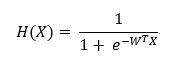
\includegraphics[scale=0.6]{4.jpg}
\end{figure}

\subsection{29/09/17}
5-2 Logistic Regression, Cost function\newline
Cost function for sigmoid function\newline

\begin{figure}[h!]
\centering
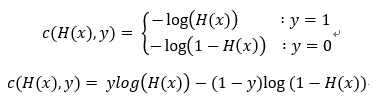
\includegraphics[scale=0.6]{5.jpg}
\end{figure}
Minimize cost – Gradient decent algorithm\newline
\begin{minted}[mathescape,
               linenos,
               numbersep=5pt,
               gobble=2,
               frame=lines,
               framesep=2mm]{python}
  #cost function
  cost = tf.reduce_mean(-tf.reduce_sum(Y*tf.log(hypothesis) + (1-Y)*tf.log(1-hypothesis)))
  #Minimize
  a = tf.Variable(0.1) #learning rate
  optimizer = tf.train.GradientDescentOptimizer(a)
  train = optimizer.minimize(cost)
\end{minted}\newline
\begin{figure}[h!]
\centering
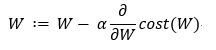
\includegraphics[scale=0.6]{6.jpg}
\end{figure}

\subsection{02/09/17}
6-1 Multinomial(Softmax)\newline
Several binomial classifications can make Multinomial classification.\newline
To classify (A, B, C), We can use 3 binomial classifications (A or not), (B or not), (C or not)\newline
\begin{figure}[h!]
\centering
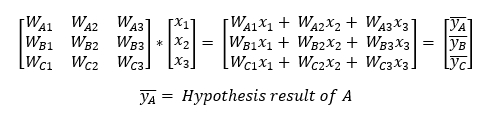
\includegraphics[scale=0.6]{7.jpg}
\end{figure}
Softmax function: substitute of Logistic function for Multinomial classification\newline

\begin{figure}[h!]
\centering
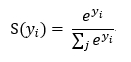
\includegraphics[scale=0.6]{8.jpg}
\end{figure}
Cost function of Softmax is Cross-Entropy \newline

\begin{figure}[h!]
\centering
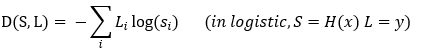
\includegraphics[scale=0.6]{9.jpg}
\end{figure}
After we find the cost function, same as logistic regression, find the minimize of cost function by using Gradient descent algorithm.\newline

\subsection{03/09/17}
6-2 Implementation Softmax classification, Tensorflow\newline
\begin{minted}[mathescape,
               linenos,
               numbersep=5pt,
               gobble=2,
               frame=lines,
               framesep=2mm]{python}
  #softmax function
  Hypothesis = tf.nn.softmax(tf.matmul(X,W) + b)

  #Cross entropy cost/loss
  Cost = tf.reduce_mean(-tf.reduce_sum(Y * tf.log(hypothesis), axis = 1))
  Optimizer = tf.train.GradientDescentOptimizer(learning_rate = 0.1).minimize(cost)

  #Testing & One-hot encoding
  a = sess.run(hypothesis, feed_dict={X: [1, 11, 7, 9]})
  print(a, sess.run(tf.arg_max(a,1)))
\end{minted}\newline

\subsection{04/09/17}
7-1 Learning rate, overfitting\newline

Learning rate\newline
1.	Large learning rate: overshooting\newline
Large steps divergence the value\newline
2.	Small learning rate: takes too long, stops at local minimum.\newline
Try several learning rates > observe the cost function, check it goes down in a reasonable rate\newline

-Overfitting\newline
*	Our model is very good with training data set(with memorization)\newline
*	Not good at test dataset or in real use\newline

-Solutions for overfitting\newline
*	More training data\newline
*	Reduce the number of features\newline
*	Regularization\newline
*	Let’s not have too big numbers in the weight.\newline
\begin{figure}[h!]
\centering
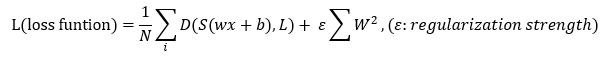
\includegraphics[scale=0.6]{10.jpg}
\end{figure}

\subsection{05/09/17}
8-1 Basic concept of Deep Learning, XOR problem\newline
Solving XOR problem : backpropagation(Paul Werbos)\newline

Big problem(1990s)\newline
*	Backpropagation just did not work well for normal neural nets with many layers\newline
*	Other rising machine learning algorithm: SVM, RandomForest\newline

Breakthrough(2006)\newline
*	Neural networks with many layers really could be trained well, if the weights are initialized in a clever way rather than randomly\newline
*	Deep machine learning methods are more efficient for difficult problems than shallow methods\newline

\subsection{06/09/17}
8-2 Backpropagation\newline
Back propagation(chain rule)\newline
\begin{figure}[h!]
\centering
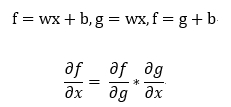
\includegraphics[scale=0.6]{11.jpg}
\end{figure}
chain rule\newline
We can simplify the neural nets with many layers. \newline

\subsection{09/09/17}
9-1 Initial weight\newline

Need to set the initial weight values wisely\newline
*	Not all 0’s\newline
*	Challenging issue\newline
*	Hinton et al. (2006)“A fast learning algorithm for Deep belief Nets”\newline

How can we use RBM to initialize weights?\newline
*	Apply the RBM idea on adjacent two layers as a pre-training step\newline
*	Continue the first process to all layers\newline
*	This will set weights\newline
*	Ex: Deep Belief Network\newline

\subsection{10/09/17}
9-2 Dropout\newline
Dropout: A simple way to prevent Neural Networks from Overfitting[Srivastava et al. 2014]\newline
“randomly set some neurons to zero in the forward pass”\newline
\begin{minted}[mathescape,
               linenos,
               numbersep=5pt,
               gobble=2,
               frame=lines,
               framesep=2mm]{python}
  #TensorFlow implementation
  Dropout_rate = tf.placeholder("float")
  _L1 = tf.nn.relu(tf.add(tf.matmul(X, W1), B1))
  L1 = tf.nn.dropout(_L1, dropout_rate)

  #Train
  Sess.run(optimizer, feed_dict={X: batch_xs, Y: batch_ys, dropout_rate: 0.7})

\end{minted}\newline

\section{Daily Report: Break}
\subsection{12/10/17 - 20/10/17}
Mid-term Exam\newline

\section{Daily Report: PyTorchZeroToAll}
\subsection{23/10/17}
-Basic concept of Machine Learning & Deep Learning\newline
1) Human Intelligence\newline
Human use inferring or prediction to decide what to do using information as inputs.\newline
2) Machine Learning & Deep Learning\newline
Also, using a lot of information about something and then infer or predict something. For example, these are 'what is number', 'what kind of shoes you were', 'where is here(using images)' etc.
We feed images and corresponding true labels(data sets) to train machine. After that, machine learn images if machine get input image then usually print output as true labels.
3) Deep Learning\newline
Deep Learning is group of algorithm that are using deep neural nets which have enormous layer.\newline
 $Deep Learning\subset Representation learning\subset Logistic regression\subset AI
 $\newline
 Deep Learning developers need to have basic algebra, probability and python.\newline
 
 
\subsection{24/10/17}
-PyTorch Overview\newline
1) PyTorch\newline
This is computing package based on Python, and it supply Tensor which is like neuron in machine.\newline
2) Install PyTorch\newline
Before installing PyTorch, install CUDA and cuDNN. CUDA is a parallel computing language and cuDNN is used to accelerate GPU.\newline
In Linux OS, we write\newline pip3 install http://download.pytorch.org/whl/cu80/torch-0.2.0.post3-cp36-cp36m-manylinux1_x86_64.whl 
pip3 install torchvision\newline on terminal to install PyTorch.\newline
-Deep Learning Abbreviation\newline
1)DNN: Deep Neural Net\newline
2)CNN: Convolution Neural Net\newline
3)RNN: Recurrent Neural Net\newline


\subsection{25/11/17}
-Types of learning\newline
1)Supervised learning\newline
Providing data sets with answers and machine train them. In the future, we use supervised learning to make model.\newline
Sequence of Learning\newline
1. Determine the subject of training\newline
2. Collect training set and test set.\newline
3. Make Model and initialize coefficients\newline
4. Run algorithm using training set(Computing training error)\newline
5. Run algorithm using test set which is separate with training set(Computing test error)\newline
6. Iterate when test error is decreasing\newline
2)Unsupervised learning\newline
Providing only data sets and machine classify data sets, so it has no evaluation of the accuracy of output.\newline
3)Reinforcement learning\newline
The machine takes action in an environment(ex. Go), and get rewards. The goal is to find the action that cause highest rewards.\newline


\subsection{26/10/17}
-Design model\newline
1.Linear model\newline
$
\hat{a} = x * w + b
$\newline
x is an input data, w is an weight, b is a bias and $y\wedge$ is the prediction of grond truth.
We start w in random value.\newline
For Updating w in our model, we calculate training loss(error) as MSE(Mean Squared Error)\newline
\begin{center}
$loss = \frac1N{\textstyle\sum_{n=1}^N}{\textstyle(}{\textstyle\hat{y_n}}{\textstyle-}{\textstyle{\scriptstyle y}_n}{\textstyle{\scriptstyle)}^2}$
 \end{center}\newline
 
 
 
\subsection{27/10/17}
-Finding weight that minimize error\newline
1. Gradient descent\newline
We initialize weight(w) randomly and use \textbf{Gradient} = $\frac{\partial loss}{\partial w}$\newline
Using gradient and step size(learning rate) update w to move in to smaller loss \newline
Loss is defined by MSE, so loss function is kind of polynomial function that has minimum value when derivative of the function is zero.\newline
\begin{center}
$w_{t+1} = w_{t}\alpha \frac{\partial loss}{\partial w}$
 \end{center}\newline
2. Setting $\alpha$(step size)\newline
If step size is too small, then w put in the local minimum not global minimum and if step size is too big, then $\alpha \frac{\partial loss}{\partial w}$ is so big that loss function and w are divergent.\newline



\subsection{30/10/17}
-Updating weight in model which has 1 or more hidden layers\newline
If network is complicated, we often are using nonlinearities between nodes. So manually computing this gradient need huge computing power and time.\newline
1. Chain Rule\newline
$f = f(g); g = g(x) \newline
\fac{df}{dx} = \fac{df}{dg}\fac{dg}{dx}$\newline
This rule divide overlapping functions and compute the gradient one by one.\newline
2. Back-propagation\newline
Caculating loss using training data is forward pass. We use loss and local gradient using divided overlapping function to get global gradient of $\frac{\partial loss}{\partial w}$\newline



\subsection{31/10/17}
-PyTorch's gradient function\newline
1. Autograd
 \begin{minted}[mathescape,
               linenos,
               numbersep=5pt,
               gobble=2,
               frame=lines,
               framesep=2mm]{python}
        w = Variable(torch.Tensor([1.0]),  requires_grad=True)
        def forward(x):
            return x * w
        def loss(x, y):
            y_pred = forward(x)
            return (y_pred - y) * (y_pred - y)

        l = loss(x_val, y_val)
        l.backward()
        w.data = w.data - 0.01 * w.grad.data
\end{minted}\newline
In PyTorch, if we set w as 'requires gradient' true and use backward() function, then we get gradient of loss automatically.\newline

\subsection{1/11/17}
-Type of Activation Functions\newline
This determine activation state(0, 1) of node by the node's input data \newline
1. Sigmoid\newline
\begin{center}$h(x) = \frac{1}{1+{e}^{-x}}$\end{center}\newline
This is one of the simple activation function. Sigmoid is logistic function. It's maximum approximate to 1 and minimum is approximate to zero.\newline
2. ReLU(Rectified Linear Unit)\newline
ReLU is h(x) = x when x is over 0, otherwise h(x) = 0. It's usually use because ReLU's derivative is so simple that h'(x) =  1 when x is over 0 otherwise h'(x) = 0.\newline
This property has another advantages. In DNN, backpropagation using sigmoid cause loss error data because it has so many hidden layers that gradient of loss need huge amonut of iterative chain rule. But ReLU protect data when running backpropagation\newline

\subsection{2/11/17}
-Type of Optimizers(1): step direction\newline
1.GD(Gradient Descent)\newline
It is check all data and find gradient at weight w position in loss function and move to most sheer direction.\newline
2.SGD(Stochastic Gradient Descent)\newline
GD is slow because of reflecting all data, so make subset data evenly and use these to move more quickly.\newline
3.Momentum\newline
Using momentum, we move to calculated step direction + a bit of last direction as momentum.\newline
4.NAG(Nestrov Accelerated Gradient)(from Momentum)\newline
First move momentum direction and then calculate move direction for move.\newline
5. Adam(from Momentum)\newline
RMSProp(in Type of Optimizers(2)) + Momentum = suitable step direction and step size.\newline
6. Nadam(from NAG and Adam)\newline
RMSProp + NAG (not Momentum)\newline

\subsection{3/11/17} 
-Type of Optimizers(2): step size\newline
1.Adagrad\newline
If the calculated step direction point to where we wasn't go, increase step size. Otherwise, decrease step size gradually.\newline
2. AdaDelta(from Adagrad)\newline
AdaDelta protect on stop when running Adagrad at where we went.\newline
3. RMSProp\newline
RMSProp block small step size dealing with each instance separately.\newline
4. Adam(from RMSProp)(in Type of Optimizers(1))\newline


\subsection{6/11/17}
-Make Binary prediction model (Pass or Fail)\newline
We plug into sigmoid from the output of the linear layer to make squash numbers between 0 to 1. In this case, if $ \hat{y} > 0.5$ than we assume that output is 1 otherwise 0.\newline With sigmoid, MSE is not work well because it's optimize for linear regression. So we need new loss function, cross entropy loss that is optimize for logistic regression and classification.\newline
\begin{center}$loss = -\frac1N{\textstyle\sum_{n=1}^N}{y}_{n} log\hat{y_n} + (1-{y_n})log(1-\hat{y_n})$\end{center}\newline
 
 
\subsection{7/11/17}
-Reading data size at once\newline
It's not efficient that we compute the gradients for all data points therefore we divide data set into small batches.\newline
1. One epoch\newline
one forward pass and on backward pass of all the training examples.\newline
2. Batch size\newline
the number of training examples in one forward/backward pass. We adjust the batch size by memory volume.\newline
3. Number of iterations\newline
It's number of passes. The one pass is one forward process + one backward process.\newline
4. Data load sequence as batches \newline
original data $->$ random shuffle $->$ making queue $->$ using queue each element as batch.\newline

\subsection{8/11/17}
-Classify data to 3 or more\newline
1. Softmax\newline
\begin{center}
            ${\sigma(\boldsymbol{z})}_{j} = \frac{{e}^{{z}_{j}}}{\sum_{k=1}^{K}{e}^{{z}_{k}}}$  
\end{center}
We use softmax with cross entropy cost function that is sum of -Ylog$\hat{Y}$. Y and $\hat{Y}$ is vector like [0.0 1.0 0.0 0.0], thus this is fit to our purpose(classification).\newline

\subsection{9/11/17}
-CNN(1)\newline
General CNN is consist of feature extraction that is convolution + subsampling and classification that is fully connected layer; Dense Net. 
1.Convolution\newline
it is going to look at only small part of image at once. So we use filter that is small than input image data. Filter moves entire image but we look at only small portion at a time.
Filter is a kind of vector, so we get output from inner product between filter and the part of image.\newline
Stride is filter's move block step. Padding is attach values at boundary of data to filter can read first pixel of image. If image hasn't padding, then filter can't read some pixel by filter size. Thus, output image size decrease.\newline
2. Activation\newline
After Convolution, we use activation function to output.
3. Max Pooling\newline
After repeating convolution + activation(ReLU) n times, we do max pooling to reduce image size. In this process, we get meta data of image. So the reduce information is small compared to decrease computation time(time complexity).\newline
4. Fully Connected layer\newline
After repeating 1,2 and 3, finally we use it some times and classify output data as softmax.\newline
\subsection{10/11/17}
-CNN(2)\newline
The addvanced mthod of CNN fine to data case by case.\newline
1. 1x1xn convolution\newline
The convolution filter is 1x1 and depth is more than n. It's control image's depth size.\newline
2. Deep Residual Learning\newline
Plaint net vulnerable to vanishing gradient. One of the solutions is using Residual Net that set up input + weight layer(convolution layer etc.) as output and then output is used as input of activation function.







\section{Application(1)}
\subsection{13/11/17 - 01/12/17}
-Deep Learning Application(1)\newline\newline
\subsubsection{Abstract}
Simple Neural Net for Iris dataset using PyTorch. Multilayer perceptron model, with one hidden layer.
\subsubsection{Keyword}
hidden layer, PyTorch, Machine Learning,Neural Net, Multilayer perceptron model.

\subsubsection{Introduction}
This is a collection of simple and easy to read program for Iris dataset classification by using PyTorch library 

\subsubsection{Method}

  SECTION 1 : Load and setup data for training\newline\newline
  the datasets separated in two files from originai datasets:\newline
  iris_train.csv = datasets for training purpose, 80 from the original data\newline
  iris_test.csv  = datasets for testing purpose, 20 from the original data\newline
  
  SECTION 2 : Build and Train Model\newline\newline
  Multilayer perceptron model, with one hidden layer.\newline
  input layer : 4 neuron, represents the feature of Iris\newline
  hidden layer : 10 neuron, activation using ReLU\newline
  output layer : 3 neuron, represents the class of Iris\newline\newline
  optimizer = stochastic gradient descent with no batch-size\newline
  loss function = categorical cross entropy\newline
  learning rate = 0.01\newline
  epoch = 500\newline
  
  SECTION 3 : Testing model\newline


\begin{minted}[mathescape,
               linenos,
               numbersep=5pt,
               gobble=2,
               frame=lines,
               framesep=2mm]{python}
               
  import pandas as pd

  #load
  datatrain = pd.read_csv('../Datasets/iris/iris_train.csv')

  #change string value to numeric
  datatrain.set_value(datatrain['species']=='Iris-setosa',['species'],0)
  datatrain.set_value(datatrain['species']=='Iris-versicolor',['species'],1)
  datatrain.set_value(datatrain['species']=='Iris-virginica',['species'],2)
  datatrain = datatrain.apply(pd.to_numeric)

  #change dataframe to array
  datatrain_array = datatrain.as_matrix()

  #split x and y (feature and target)
  xtrain = datatrain_array[:,:4]
  ytrain = datatrain_array[:,4]

  import torch
  import torch.nn as nn
  import torch.nn.functional as F
  from torch.autograd import Variable
  torch.manual_seed(1234)

  #hyperparameters
  hl = 10
  lr = 0.01
  num_epoch = 500

  #build model
  class Net(nn.Module):

      def __init__(self):
          super(Net, self).__init__()
          self.fc1 = nn.Linear(4, hl)
          self.fc2 = nn.Linear(hl, 3)

      def forward(self, x):
          x = F.relu(self.fc1(x))
          x = self.fc2(x)
          return x
  net = Net()

  #choose optimizer and loss function
  criterion = nn.CrossEntropyLoss()
    optimizer = torch.optim.SGD(net.parameters(), lr=lr)

  #train
  for epoch in range(num_epoch):
      X = Variable(torch.Tensor(xtrain).float())
      Y = Variable(torch.Tensor(ytrain).long())

      #feedforward - backprop
      optimizer.zero_grad()
      out = net(X)
      loss = criterion(out, Y)
      loss.backward()
      optimizer.step()

      if (epoch) % 50 == 0:
          print ('Epoch [%d/%d] Loss: %.4f' 
                     %(epoch+1, num_epoch, loss.data[0]))

  #load
  datatest = pd.read_csv('../Datasets/iris/iris_test.csv')

  #change string value to numeric
  datatest.set_value(datatest['species']=='Iris-setosa',['species'],0)
  datatest.set_value(datatest['species']=='Iris-versicolor',['species'],1)
  datatest.set_value(datatest['species']=='Iris-virginica',['species'],2)
  datatest = datatest.apply(pd.to_numeric)

  #change dataframe to array
  datatest_array = datatest.as_matrix()

  #split x and y (feature and target)
  xtest = datatest_array[:,:4]
  ytest = datatest_array[:,4]

  #get prediction
  X = Variable(torch.Tensor(xtest).float())
  Y = torch.Tensor(ytest).long()
  out = net(X)
  _, predicted = torch.max(out.data, 1)

  #get accuration
  print('Accuracy of the network %d %%' % (100 * torch.sum(Y==predicted) / 30))
\end{minted}

\newline\newline\newline

\section{Application(2)}
\subsection{04/12/17 - 27/12/17}
-Deep Learning Application(2)\newline\newline
\subsubsection{Abstract}
We classify given real image data correctly using Resnet50 with supervise learning.
\subsubsection{Keyword}
DNN, Supervised Learning, Machine Learning, Resnet50, Hymenoptera.

\subsubsection{Introduction}
Ants are similar to bees besides wings. So we classify data to ant or bee image using labeled data. In this study, we use supervised learning and Resnet50 that has 50 layers of residual structure.

\subsubsection{Method}
\paragraph{Resnet50}
\newline
\newline
 
\begin{figure}[h!]
\centering
\includegraphics[scale=0.4,left]{residual_building_block.png}
\caption{Residual network structure}
\label{fig:resnet}
\end{figure}
 
The Resnet use previous output as input and previous ouput + activated input as output[Figure 1]. So it has much more characteristic than plain net which hasn't residual edge. In [Figure 1]. We recognize that F(x) and x size are same because each of these is vector.\newline

\paragraph{Source Code}
\newline
 \newline Basic model setting as follows.\newline
Input: hymenoptera data\newline
Output: classified hymenoptera data\newline
Initial condition: labeled data\newline
Final condition: epoch 25 times\newline
\begin{minted}[mathescape,
               linenos,
               numbersep=5pt,
               gobble=2,
               frame=lines,
               framesep=2mm]{python}
               
def train_model(model, criterion, optimizer, scheduler, num_epochs=25):
    since = time.time()

    best_model_wts = model.state_dict()
    best_acc = 0.0

    for epoch in range(num_epochs):
        print('Epoch {}/{}'.format(epoch, num_epochs - 1))
        print('-' * 10)

        # Each epoch has a training and validation phase
        for phase in ['train', 'val']:
            if phase == 'train':
                scheduler.step()
                model.train(True)  # Set model to training mode
            else:
                model.train(False)  # Set model to evaluate mode

            running_loss = 0.0
            running_corrects = 0

            # Iterate over data.
            for data in dataloaders[phase]:
                # get the inputs
                inputs, labels = data

                # wrap them in Variable
                if use_gpu:
                    inputs = Variable(inputs.cuda())
                    labels = Variable(labels.cuda())
                else:
                    inputs, labels = Variable(inputs), Variable(labels)

                # zero the parameter gradients
                optimizer.zero_grad()

                # forward
                outputs = model(inputs)
                _, preds = torch.max(outputs.data, 1)
                loss = criterion(outputs, labels)

                # backward + optimize only if in training phase
                if phase == 'train':
                    loss.backward()
                    optimizer.step()

                # statistics
                running_loss += loss.data[0]
                running_corrects += torch.sum(preds == labels.data)

            epoch_loss = running_loss / dataset_sizes[phase]
            epoch_acc = running_corrects / dataset_sizes[phase]

            print('{} Loss: {:.4f} Acc: {:.4f}'.format(
                phase, epoch_loss, epoch_acc))

            # deep copy the model
            if phase == 'val' and epoch_acc > best_acc:
                best_acc = epoch_acc
                best_model_wts = model.state_dict()

        print()

    time_elapsed = time.time() - since
    print('Training complete in {:.0f}m {:.0f}s'.format(
        time_elapsed // 60, time_elapsed % 60))
    print('Best val Acc: {:4f}'.format(best_acc))

    # load best model weights
    model.load_state_dict(best_model_wts)
    return model
\end{minted}

\newline We use resnet50 to training model. Before this, first we divied 2 types of data as folder name(ants, bees).\newline
\begin{center}$ H = -y log \hat{y} -(1-y)log(1-\hat{y})$\end{center}\newline
We calculate loss using cross entropy function H for update weight.\newline


\subsubsection{Result and Conclusion}
The best accuracy is 93.46 percent. We use various type of ants and bees, but the accuracy is very high. When we train model without hidden layer, it's difficult to find global minimum position. So we know the power of hidden layers.\newline
In future, we run additional model learing in various the number of hidden layers and data to get the perfect number of hidden layer about data size.

\end{CJK}
\end{document}